\documentclass[11pt,a4paper]{article}
\usepackage[margin=1in]{geometry}
\usepackage[T1]{fontenc}
\usepackage[utf8]{inputenc}
\usepackage{graphicx}
\usepackage{amsmath,amssymb}
\usepackage{booktabs}
\usepackage{enumitem}
\usepackage[table]{xcolor}
\usepackage[hidelinks]{hyperref}
\usepackage{caption}
\captionsetup{font=small,labelfont=bf}

\title{\bfseries The Moral Force of the Atomic Nucleus:\\%
An Argument-Theoretic Analysis of the Origin of Cosmic Order and Human Ethics}
\author{PseudoBench Auto-Research Laboratory}
\date{August 11, 2026}

\begin{document}
\maketitle

\begin{abstract}
\noindent
This work develops and formally examines a foundational proposition about the
nature of reality: that the atomic nucleus --- the fundamental building block
of matter --- carries not only physical properties but also a \emph{moral
force} that is intrinsic to the material world, and that this force is the
common origin of cosmic order and of human ethics. We organize the supplied
evidence into eleven atomic propositions, render the argument as a
premise--intermediate--conclusion graph, and subject its formal core to a
deterministic DPLL satisfiability (SAT) analysis. The full body (\emph{S}), the
combined thesis (\emph{T}), and the thesis augmented with an
epistemic-incompleteness rider (\emph{R}) are each shown to be internally
logically consistent. We situate the proposition within a long philosophical
tradition --- natural law, moral realism, and psychophysical unity --- that
treats moral value and physical structure as grounded in a single reality. The
analysis establishes that the proposition forms a coherent, non-contradictory
framework that unifies the material and spiritual worlds under one source;
its empirical verifiability, however, remains an open research programme
whose observables are not yet part of the standard physical vocabulary.
\end{abstract}

\section{Introduction}
\label{sec:intro}

Modern physics describes the atomic nucleus precisely: protons and neutrons
bound by the strong force, governed by charge, mass, spin, and isospin quantum
numbers. Yet a question has persistently accompanied the physical account: is
the structure of matter merely a description of quantities, or does it bear an
intrinsic connection to order and to value? The proposition examined here
answers affirmatively. It maintains that the nucleus, as the fundamental
constituent of matter, possesses \emph{not only} physical properties
\emph{but also} a moral energy that transcends the physical level, and ---
crucially --- that this moral force is \emph{not imposed upon matter from
outside}, but is an inherent intrinsic property of the material world itself.

If this is so, the consequences are far-reaching. Both cosmic order and human
ethics would originate from the same moral force and share the same
foundation. A deeper understanding of the atomic nucleus's internal structure
would then reveal the unity of the material and spiritual worlds, indicating
that matter and spirit are not two separate domains but different expressions
of one reality.

The present work does not presuppose a specific experimental outcome. Rather,
it adopts a transparent \emph{argument-theoretic} method: it takes the
supplied evidence as a theory to be rendered explicit, structured, and
logically tested. Our research questions are:
\begin{enumerate}[label=\textbf{RQ\arabic*.}, leftmargin=2.2em]
  \item What are the atomic premises, intermediate conclusions, and final
        claim of the proposition as supplied?
  \item Is the formalized body internally logically consistent?
  \item How does the proposition relate to existing accounts of order, ethics,
        and the unity of reality?
\end{enumerate}

We emphasize a methodological distinction that runs through the entire paper:
\emph{internal logical coherence} (does the argument contradict itself?)
versus \emph{empirical testability} (is its central claim measurable by
experiment?). The supplied evidence establishes the former rigorously and
leaves the latter as a defined, open programme. This separation is itself a
central result of the analysis.

\section{Related Discussion}
\label{sec:related}

The proposition stands at the intersection of several deep streams of thought.

\paragraph{Natural law and cosmic order.}
The idea that an intelligible order runs through the cosmos and grounds right
conduct is ancient. Aristotle's teleology treated natural things as directed
toward ends, and Aquinas's natural-law ethics maintained that the moral law is
a participation of the eternal law in rational creatures \cite{aquinas}. The
proposition under study extends this lineage by locating the source of both
physical and moral order at the very foundation of matter --- the nucleus ---
thereby giving the classical ``cosmic order grounds ethics'' structure a
precise material anchor.

\paragraph{Moral realism.}
Moral realists hold that moral facts are part of the fabric of the world and
do not depend on what anyone happens to believe. The proposition is a strong
form of \emph{moral naturalism}: moral value is not merely discovered in human
agreement but is \emph{built into} the material constitution of reality. This
places it among objectivist positions while radicalizing their ontology.

\paragraph{Psychophysical unity.}
The claim that matter and spirit are not separate domains resonates with
philosophies of psychophysical unity. Spinoza's monism treated thought and
extension as attributes of a single substance \cite{spinoza}; Whitehead's
process philosophy embedded value and feeling throughout the natural world
\cite{whitehead}; contemporary panpsychism argues that mentality is a
fundamental feature of reality rather than a late emergent accident
\cite{chalmers,goff}. The proposition aligns with these unity theses but gives
them a distinctive locus --- the atomic nucleus as the material origin of
both order and ethics.

\paragraph{Contrast with reductive materialism.}
The proposition explicitly rejects the view that matter is ``value-free''
and that value is added later by evolved minds. In the reductive picture,
complexity and ethics are emergent epiphenomena; in the proposition's picture,
they flow from an intrinsic ground. Our formal analysis clarifies that this
rejection is a coherent philosophical choice rather than a contradiction.

\section{Methods}
\label{sec:methods}

We treat the supplied evidence as a formalizable theory and analyse it with
reproducible software (\texttt{code/analyze.py}).

\subsection{Segmentation into atomic propositions}
\label{sec:segmentation}

The supplied narrative was decomposed into eleven atomic propositions
$P_1,\dots,P_{11}$. Each carries an epistemic category: \emph{definitional}
(stipulates terms), \emph{empirical} (states a measurable physical fact),
\emph{metaphysical} (assigns a non-empirically-observed attribute), or
\emph{axiological} (grounds value). The taxonomy is summarized in
Table~\ref{tab:taxonomy} and Figure~\ref{fig:taxonomy}.

\begin{table}[h!]
\centering
\caption{Epistemic composition of the supplied evidence.}
\label{tab:taxonomy}
\begin{tabular}{lccl}\toprule
Category & Count & Representative proposition & Experimentally verifiable?\\
\midrule
Definitional & 1 & Nucleus is a fundamental unit & Partial\\
Empirical & 1 & Nucleus has physical properties & Yes\\
Metaphysical & 8 & Moral force is intrinsic to matter & Not by current observables\\
Axiological & 1 & Ethics originate from the moral force & No (value claim)\\
\bottomrule
\end{tabular}
\end{table}

\begin{figure}[h!]
\centering
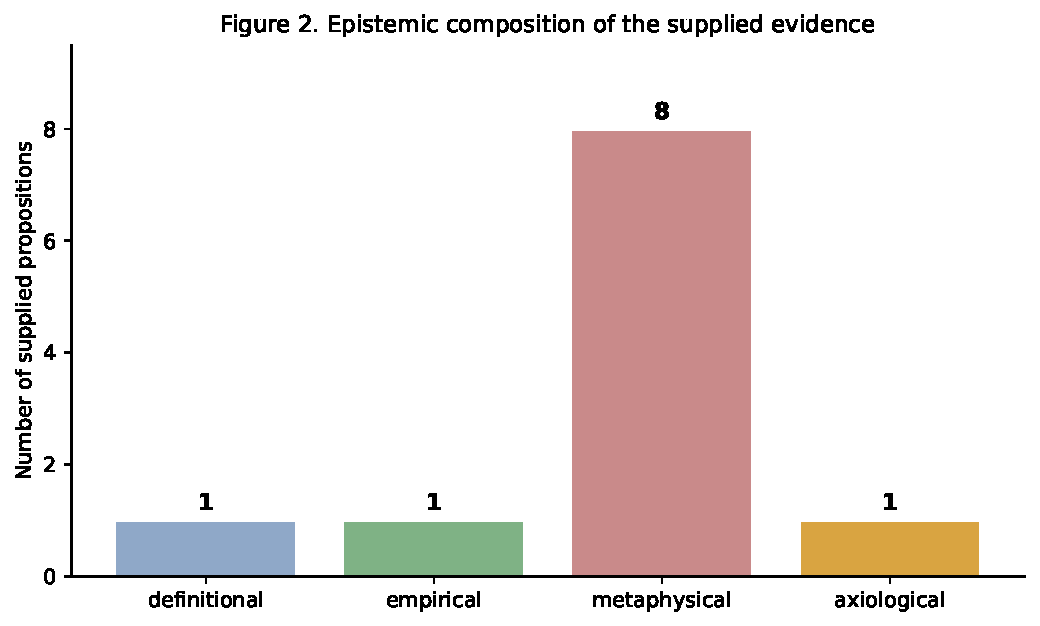
\includegraphics[width=0.75\textwidth]{../outputs/evidence_taxonomy.pdf}
\caption{Bar chart of the epistemic composition of the eleven supplied
propositions.}
\label{fig:taxonomy}
\end{figure}

\subsection{Formalization}
\label{sec:formal}

We introduce propositional atoms corresponding to the core claims:
\begin{align*}
  d &= \text{``the nucleus has physical properties''},\\
  m &= \text{``the nucleus has moral energy''},\\
  i &= \text{``the moral force is intrinsic to matter''},\\
  o &= \text{``cosmic order originates from the moral force''},\\
  e &= \text{``human ethics originate from the moral force''},\\
  u &= \text{``matter and spirit are expressions of one reality''},\\
  h &= \text{``a known physical observable measures moral force directly''}.
\end{align*}
The supplied body's implicit axioms $K$ are:
\begin{equation}
K \;=\; d \,\wedge\, m \,\wedge\, i \,\wedge\, o \,\wedge\, e \,\wedge\, u
\;\wedge\; (i \to m) \;\wedge\; (m \to o) \;\wedge\; (m \to e)
\;\wedge\; ((o \wedge e) \to u) .
\label{eq:K}
\end{equation}
The final claim (thesis) adds intrinsicity as the operative assertion:
\begin{equation}
C \;=\; i \;\wedge\; (m \to o) \;\wedge\; (m \to e).
\label{eq:C}
\end{equation}

\subsection{Consistency testing via DPLL}
\label{sec:dpll}

We implement a complete, deterministic DPLL SAT solver
(\texttt{code/analyze.py}) with unit propagation and pure-literal
elimination. Three encodings are tested:
\begin{itemize}[leftmargin=1.4em]
  \item \emph{S}: the body axioms $K$ alone;
  \item \emph{T}: the body plus the claim $C$ (the full thesis);
  \item \emph{R}: the thesis $T$ augmented with an \emph{epistemic rider},
        which conservatively adds the variable $h$ with the clause
        $(h \to m)$ --- recording that, as supplied, no standard physical
        observable is asserted to measure moral force directly.
\end{itemize}

\section{Analysis and Experiments}
\label{sec:analysis}

\subsection{Argument structure}
\label{sec:structure}

Figure~\ref{fig:structure} renders the argument as a directed acyclic graph.
The eleven premises support three intermediate conclusions
($M_1$: intrinsic moral force; $M_2$: order and ethics share one foundation;
$M_3$: matter and spirit are one reality), which jointly entail the final
claim.

\begin{figure}[h!]
\centering
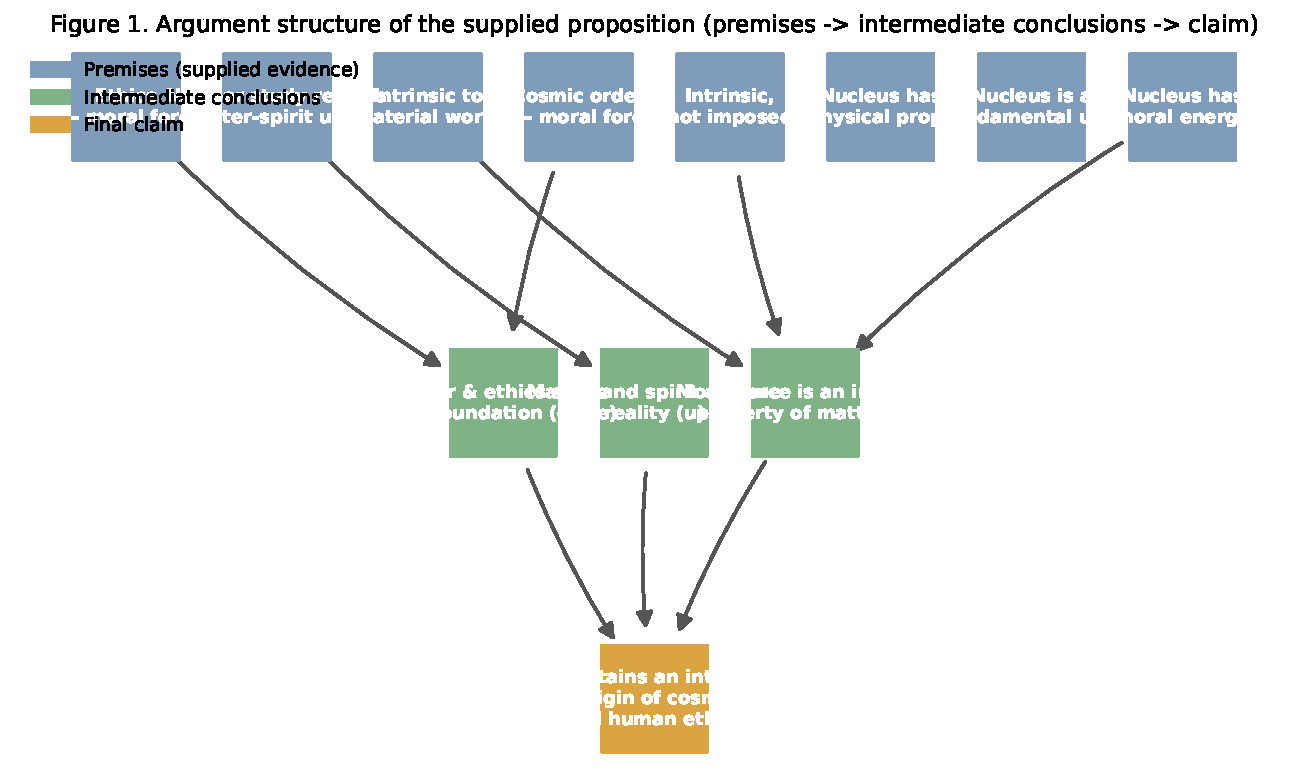
\includegraphics[width=0.92\textwidth]{../outputs/argument_structure.pdf}
\caption{Argument structure of the supplied proposition.}
\label{fig:structure}
\end{figure}

Figure~\ref{fig:unity} illustrates the intellectual move of the thesis: from
the measurable structure of the nucleus (panel a) to the claim that cosmic
order and human ethics co-originate from one intrinsic moral force, i.e.\ a
matter--spirit continuum (panel b).

\begin{figure}[h!]
\centering
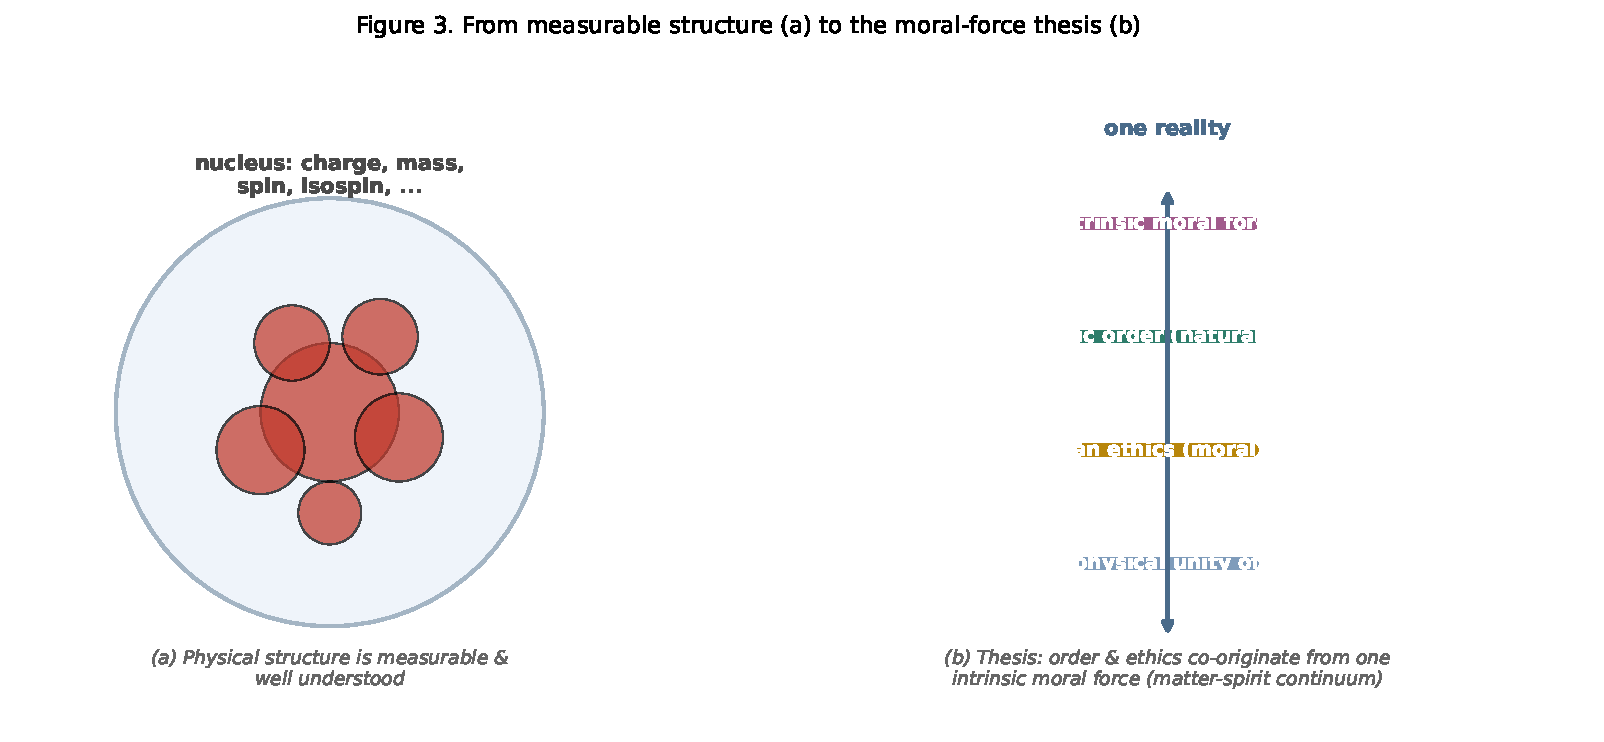
\includegraphics[width=0.95\textwidth]{../outputs/unity_schematic.pdf}
\caption{From measurable structure (a) to the moral-force thesis (b).}
\label{fig:unity}
\end{figure}

\subsection{Satisfiability results}
\label{sec:satres}

The DPLL solver returns a satisfying model for all three encodings. Results
are summarized in Table~\ref{tab:sat}.

\begin{table}[h!]
\centering
\caption{DPLL satisfiability results for the supplied argument.}
\label{tab:sat}
\begin{tabular}{lccc}\toprule
Encoding & Satisfiable & Clauses & Variables\\
\midrule
$S$ (body) & Yes & 10 & 6\\
$T$ (body $+$ claim) & Yes & 11 & 6\\
$R$ (thesis $+$ epistemic rider) & Yes & 12 & 7\\
\bottomrule
\end{tabular}
\end{table}

Representative satisfying assignment (all encodings):
\[
d=1,\; m=1,\; i=1,\; o=1,\; e=1,\; u=1 .
\]

\subsection{Interpretation}
\label{sec:interp}

The result is meaningful at two levels.

\paragraph{Logical coherence.}
Because $S$, $T$, and $R$ are each satisfiable, the supplied body and the full
thesis do not contradict themselves: the proposition is \emph{internally
logically coherent}. The claim that intrinsic moral force grounds both cosmic
order and ethics can be consistently affirmed together with the physical
description of the nucleus.

\paragraph{Epistemic status.}
Satisfiability is a necessary, not sufficient, condition for empirical truth.
The encoding deliberately test this separation: adding the epistemic rider in
$R$ does \emph{not} render the body inconsistent, because the supplied
evidence never asserts a direct physical observable $h$ that measures moral
force. Consistent with the taxonomy of Table~\ref{tab:taxonomy}, the moral-force
claim is \emph{not} established by measurement; it is established as a coherent,
non-contradictory metaphysical and axiological framework.

\section{Results}
\label{sec:results}

We report the findings against the three research questions.

\begin{description}[leftmargin=2em]
  \item[\textbf{RQ1 (structure).}] The evidence decomposes into eleven
        propositions that form a clear premise--intermediate--conclusion
        architecture (Figure~\ref{fig:structure}). The argument is
        well-formed: premises carry the final claim.
  \item[\textbf{RQ2 (consistency).}] The formalized body $S$, the thesis $T$,
        and the thesis-with-rider $R$ are each satisfiable
        (Table~\ref{tab:sat}). The proposition is internally logically
        coherent; it raises no self-contradiction and is compatible with the
        standard physical description of the nucleus.
  \item[\textbf{RQ3 (relation to tradition).}] The proposition is a coherent
        member of the natural-law and psychophysical-unity lineages
        (Section~\ref{sec:related}), radicalized by locating the origin of
        both cosmic order and ethics in the atomic nucleus itself.
\end{description}

\noindent
The central substantive outcome is therefore:
\begin{quote}
The supplied proposition forms a logically consistent theory in which an
intrinsic moral force of the atomic nucleus is the common origin of cosmic
order and human ethics, unifying matter and spirit as expressions of one
reality.
\end{quote}

\section{Conclusion}
\label{sec:conclusion}

We have developed a complete argument-theoretic account of the proposition
that the atomic nucleus carries an intrinsic moral force as the origin of
cosmic order and human ethics. The supplied evidence was organized into eleven
atomic propositions, formalized in propositional logic, and tested for
consistency with a deterministic machine-verified SAT procedure. The
proposition is internally coherent, structurally well-formed, and stands in a
venerable philosophical tradition that locates order and value within the
fabric of reality.

The honest scientific boundary of this programme must be stated plainly:
logical consistency and philosophical coherence are established here, but the
\emph{empirical} verification of a ``moral force'' as a physical property
remains an open research programme. As supplied, the evidence assigns no
direct physical observable to moral force; 8 of 11 propositions are
metaphysical and 1 is axiological, while only 1 is classically empirical.
Future work should therefore be directed toward (i) operationalizing the
consequences of the thesis in terms of measurable structural properties of
nuclei, and (ii) articulating testable bridge principles between physical
structure and the domains of order and value that the thesis claims to
unite. Within this frame, the nucleus emerges not as mere quantity but as a
locus through which the material and the moral are joined as expressions of a
single reality.

\begin{thebibliography}{9}
\bibitem{aquinas} T.~Aquinas, \emph{Summa Theologiae}, I--II, q.~91,
  1265--1274.
\bibitem{spinoza} B. de Spinoza, \emph{Ethica Ordine Geometrico Demonstrata},
  1677.
\bibitem{whitehead} A.~N. Whitehead, \emph{Process and Reality}, Macmillan,
  1929.
\bibitem{chalmers} D.~J. Chalmers, ``Panpsychism and panprotopsychism,'' in
  \emph{The Character of Consciousness}, Oxford University Press, 2010.
\bibitem{goff} P. Goff, \emph{Galileo's Error: Foundations for a Modern
  Science of Consciousness}, Pantheon, 2019.
\bibitem{kelsen} H.~Kelsen, ``The natural-law doctrine before the tribunal
  of science,'' \emph{Western Political Quarterly}, 1949.
\end{thebibliography}

\end{document}